\subsection{Analisis Kebutuhan Sistem}

% bingung nulis apa lagi disini
Pada bagian \ref{subsec:analisis-alternatif-solusi}, telah disimpulkan pilihan alternatif yang akan digunakan dalam membangun sistem. Alternatif-alternatif solusi yang digunakan akan menjadi komponen yang saling berinteraksi dalam sistem Smart Contract Discovery untuk menyediakan fungsionalitas yang terpadu. Pada bagian ini akan diuraikan lebih lanjut mengenai sistem yang akan dibangun sehingga dapat memberikan panduan dalam fase pengembangan sistem. Penjelasan ini mencakup deskripsi sistem, karakteristik pengguna, kebutuhan fungsional, serta model use case yang akan digunakan dalam sistem.

\subsubsection{Deskripsi Sistem}
% penjelasan gambaran umum sistem, komponen utamanya apa aja
% buat diagram UML gambaran umum
% Jelaskan tujuan utama sistem (misalnya: "Membangun sistem pencarian smart contract berbasis semantik untuk meningkatkan efisiensi pengembangan dApps").

Solusi yang akan dikembangkan adalah sebuah sistem Smart Contract Discovery yang bertujuan untuk menjadi \textit{platform} pencarian Smart Contract dalam Blockchain Ethereum berbasis semantik. Sistem akan dibagi menjadi beberapa komponen utama yang saling berinteraksi untuk menyediakan fungsionalitas yang terpadu. Komponen utama sistem dapat dibagi sebagai berikut:

\begin{enumerate}
	\item Komponen Ekstraksi Data (Ethereum Archive Node dan eth2dgraph)
	\item Komponen Penyimpanan Data (DgraphDB dan Vector Database)
	\item Komponen \textit{Semantic Enrichment} (Smart Contract Enricher)
	\item Komponen Antarmuka Pengguna
\end{enumerate}

\begin{figure}[ht]
	\centering
	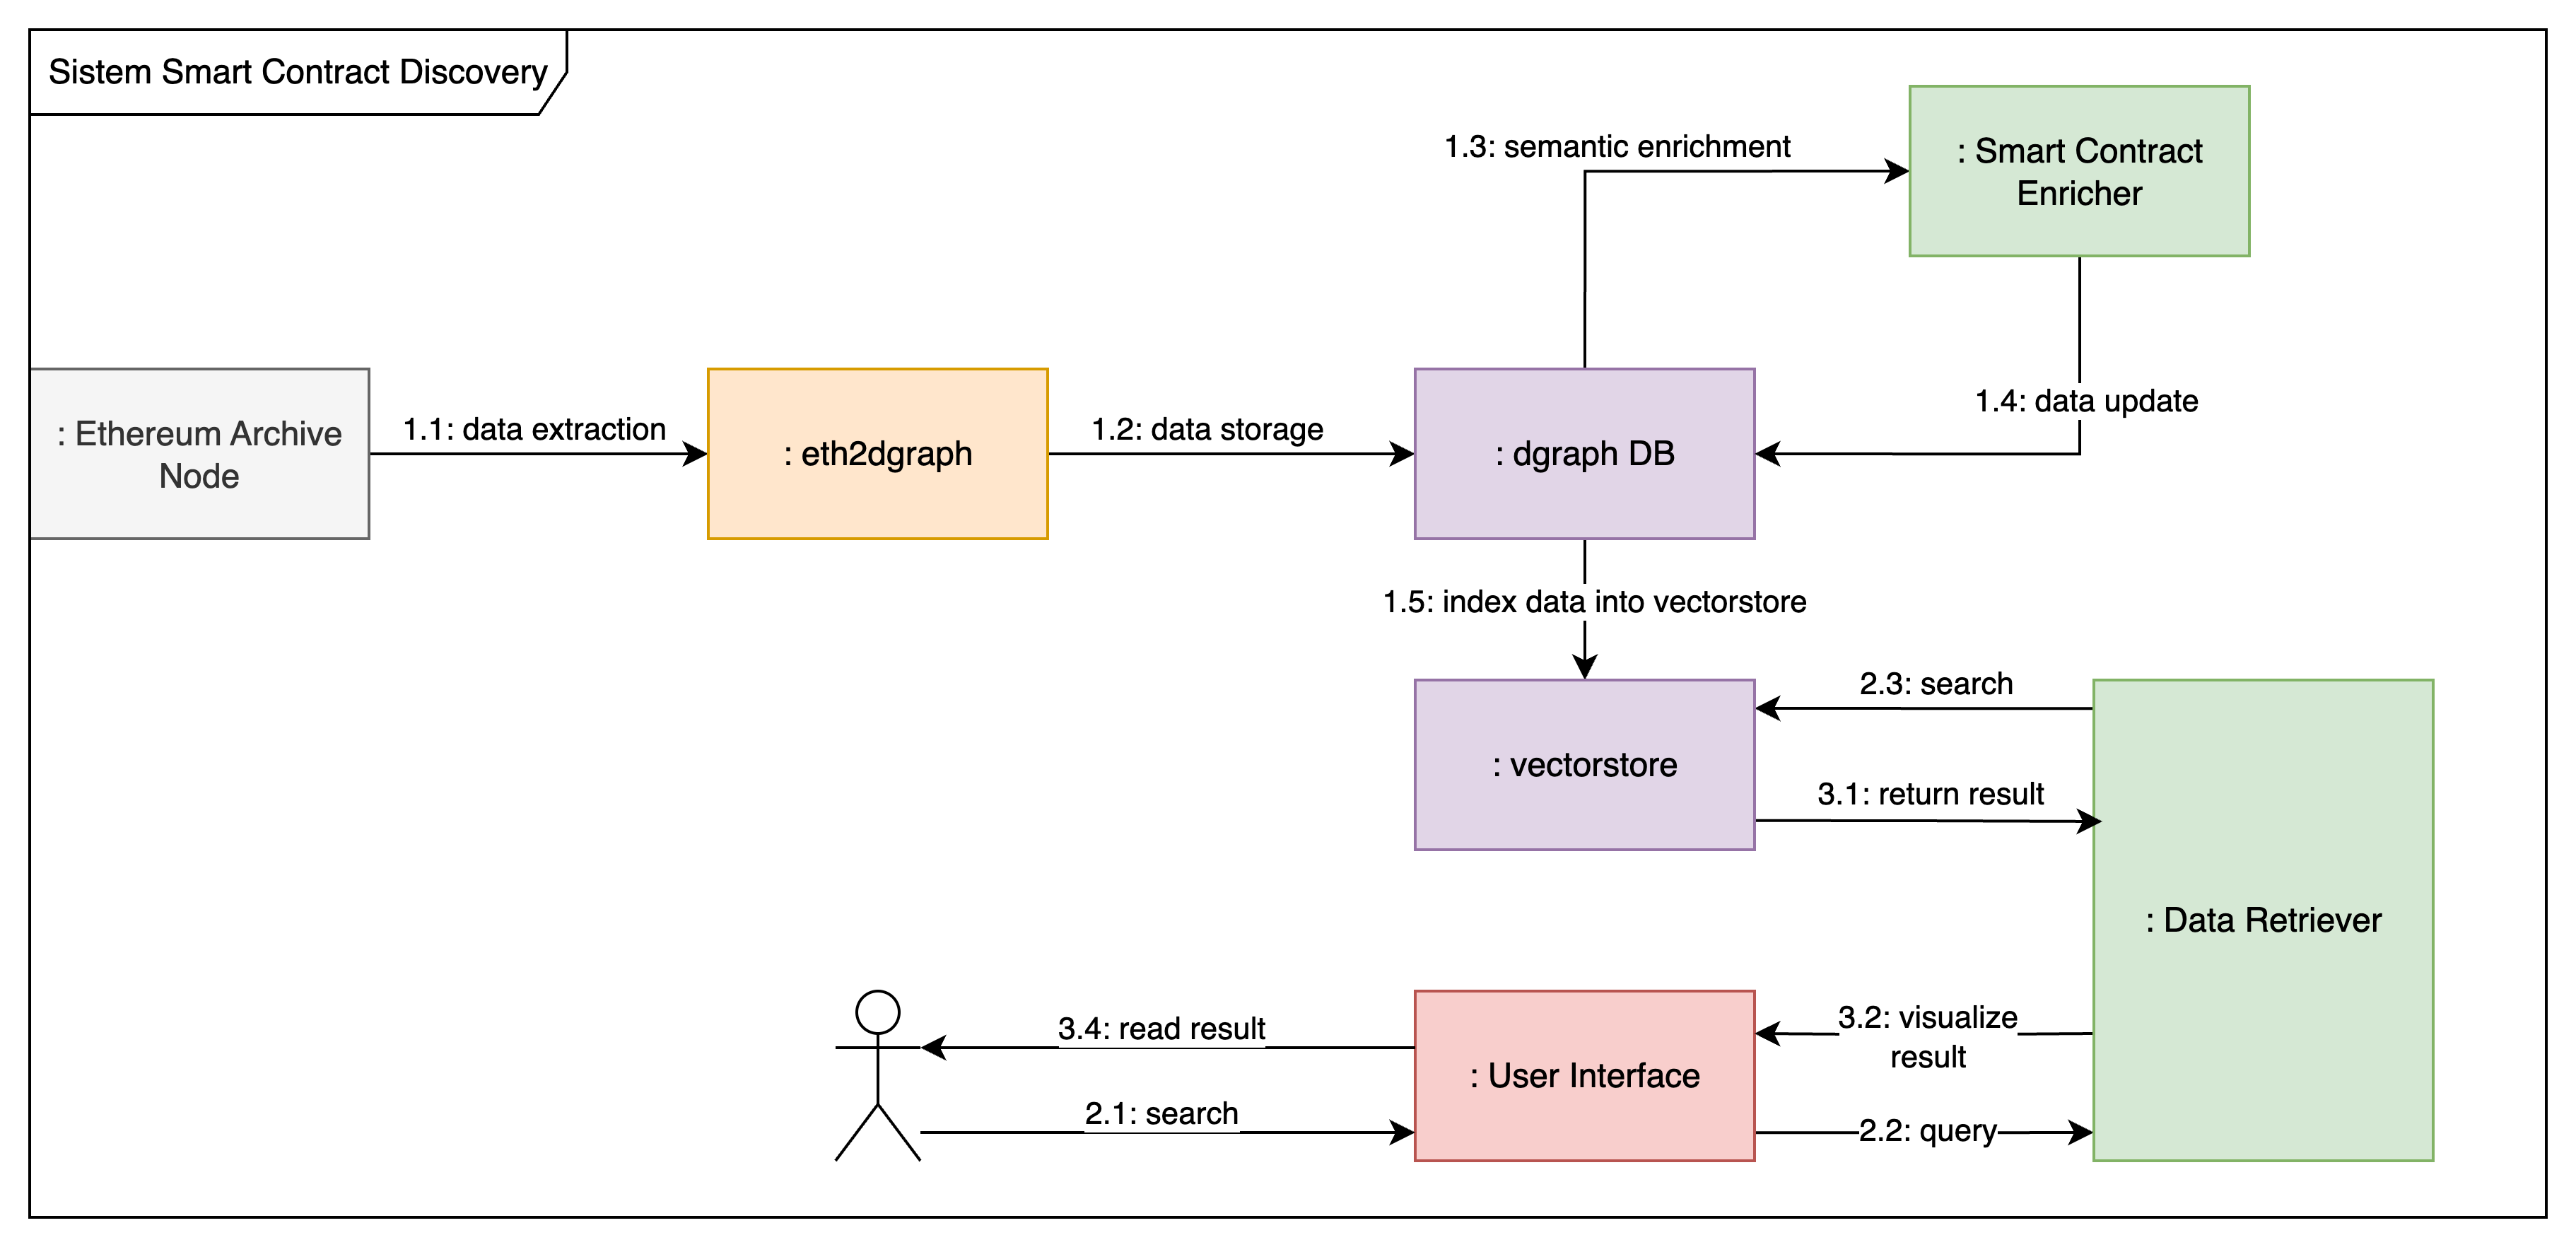
\includegraphics[width=1\textwidth]{resources/chapter-3/komponen-utama-new.png}
	\caption{Gambaran Umum Interaksi Komponen Utama Sistem}
	\label{image:komponen-sistem}
\end{figure}

\begin{figure}[ht]
	\centering
	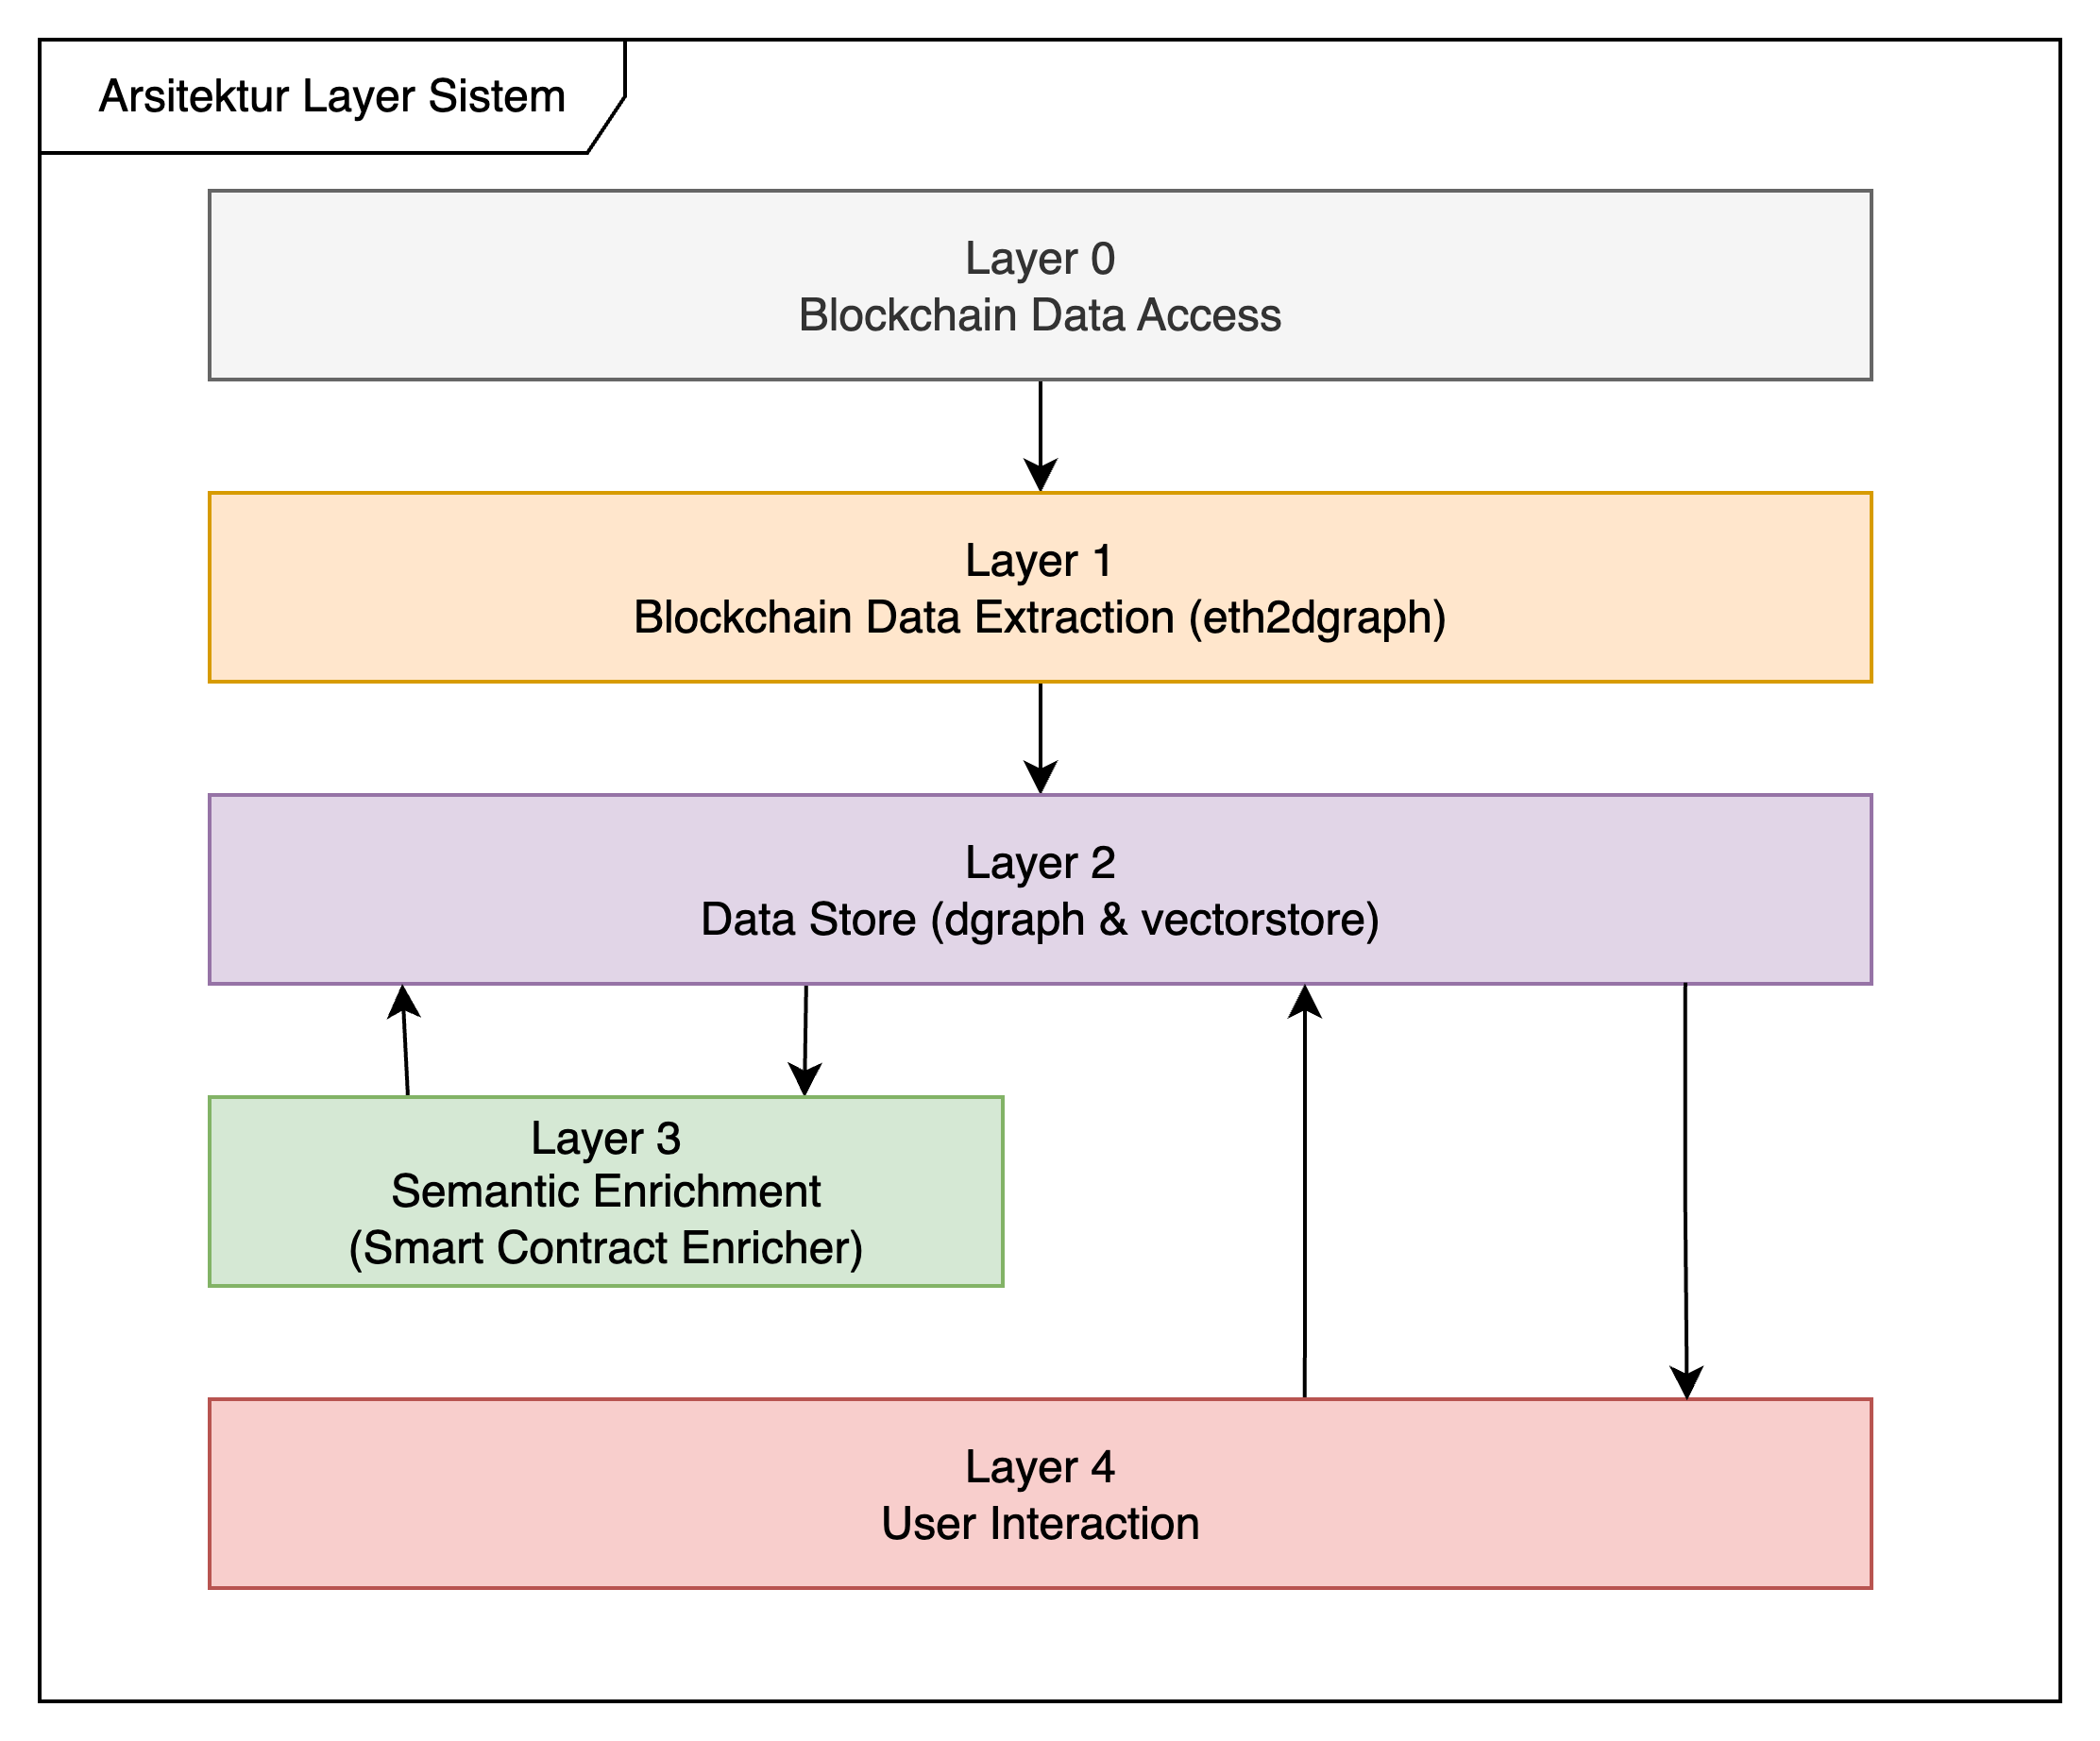
\includegraphics[width=0.7\textwidth]{resources/chapter-3/layer-arsitektur-new.png}
	\caption{Gambaran Arsitektur Layer Sistem}
	\label{image:layer-arsitektur}
\end{figure}

% Ethereum Archive Node → eth2dgraph (ekstraksi) → Dgraph (penyimpanan) → LLM (semantic enrichment) → Dgraph (update) → RAG (query).  

Gambar \ref{image:komponen-sistem} dan gambar \ref{image:layer-arsitektur} menunjukkan gambaran umum alur kerja sistem. Sistem ini akan melakukan ekstraksi data dari Ethereum Archive Node menggunakan \textit{eth2dgraph} dan menyimpannya dalam Dgraph. Setelah itu, sistem akan melakukan \textit{semantic enrichment} menggunakan LLM untuk memperkaya deskripsi dan metadata Smart Contract, lalu memperbarui data di Dgraph. Sebelum data dapat dilakukan query, akan dilakukan indexing data menjadi bentuk vector embeddings dan disimpan di dalam Vector Database. Terakhir, sistem akan menggunakan \textit{cosine similarity} atau disebut juga \textit{semantic similarity} untuk melakukan pencarian berdasarkan kebutuhan pengguna.

\subsubsection{Proses Semantic Enrichment}

Proses \textit{Semantic Enrichment} yang terdapat pada poin 1.3 pada gambar \ref{image:komponen-sistem} dapat dibagi menjadi empat bagian, yaitu proses penerapan skema sebagai \textit{template} \textit{enrichment} pada data sebelum data diproses, proses pengambilan data dari Dgraph, proses data \textit{enrichment} menggunakan LLM, dan proses \textit{update} data ke dalam Dgraph.
Proses ini akan dilakukan secara berulang-ulang hingga semua data yang ada di Dgraph terproses. Proses ini akan menghasilkan deskripsi semantik dari data sehingga dapat digunakan untuk melakukan pencarian berbasis semantik. Setelah proses \textit{enrichment} selesai, data akan disimpan kembali ke dalam Dgraph.

\begin{figure}[ht]
	\centering
	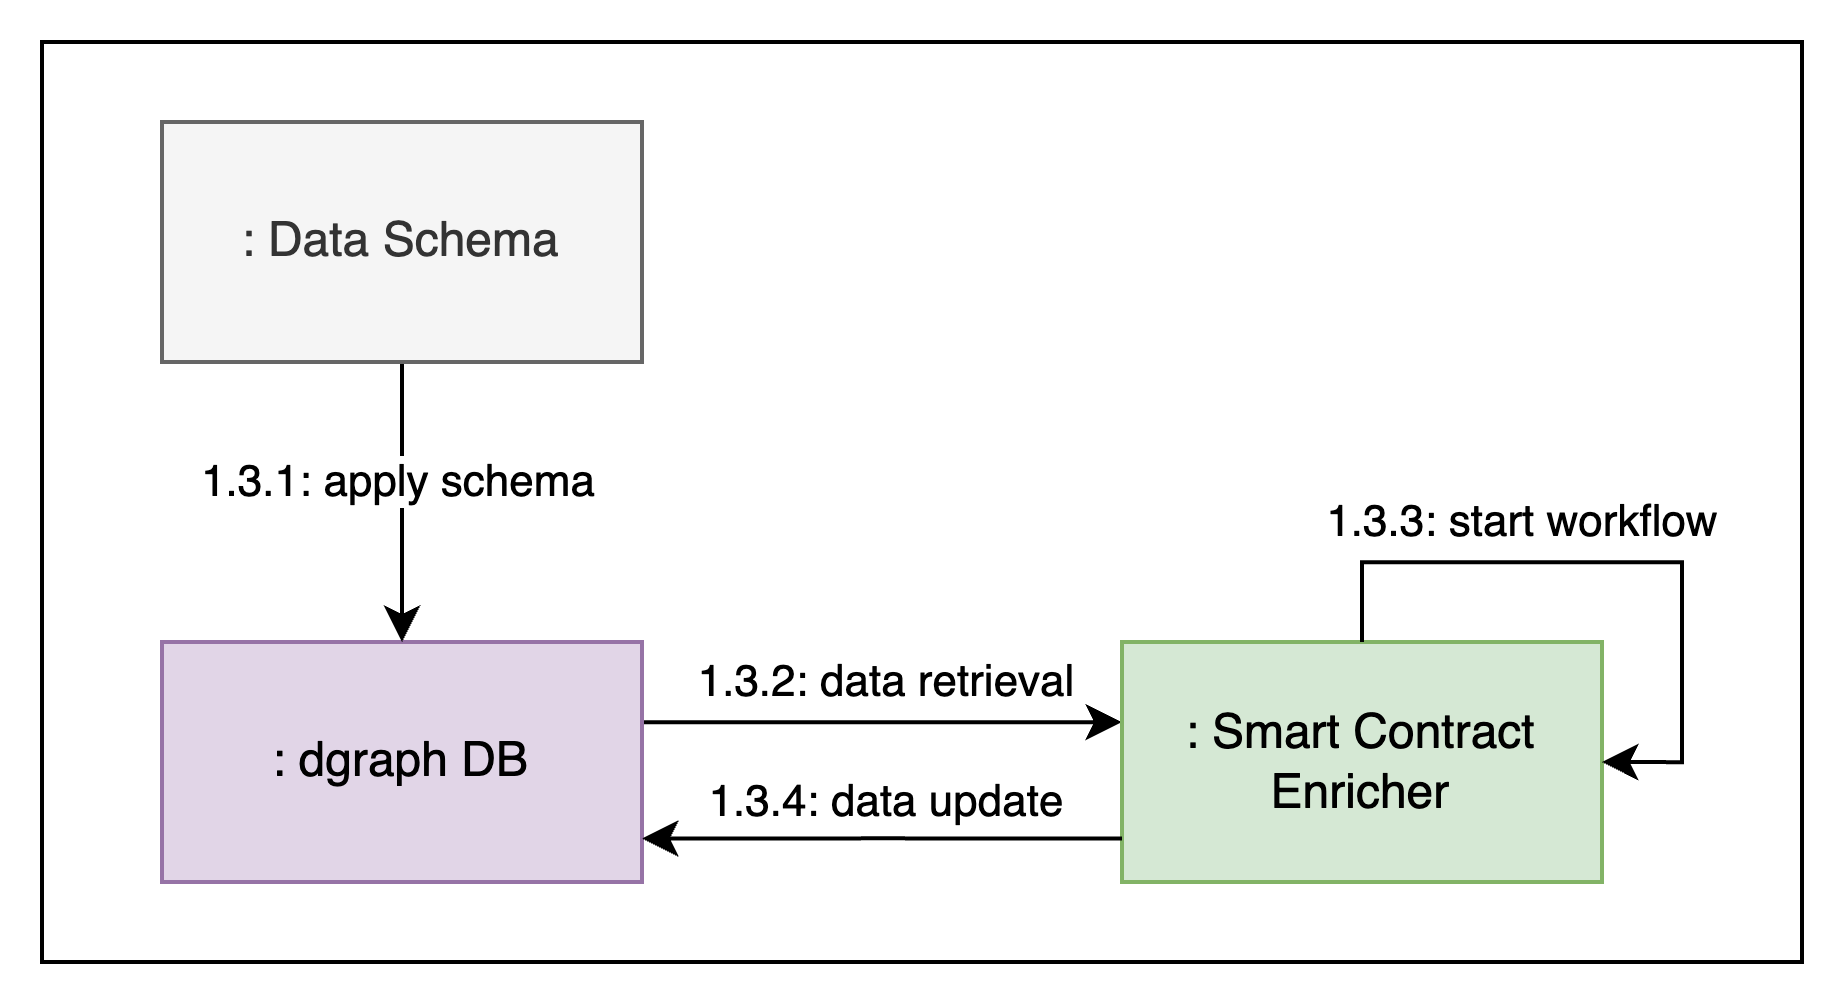
\includegraphics[width=1\textwidth]{resources/chapter-3/proses-semantik-enrichment.png}
	\caption{Proses \textit{Semantic Enrichment}}
	\label{image:proses-enrichment}
\end{figure}

\subsubsection{Skema Enriched Data}

Skema data yang akan digunakan untuk menyimpan data hasil \textit{enrichment} dapat dilihat pada lampiran \ref{appendix:skema-data}. Skema ini akan digunakan sebagai \textit{template} dan diterapkan pada DgraphDB untuk melakukan \textit{enrichment} data Smart Contract yang ada di Dgraph. Skema ini akan digunakan untuk menyimpan data hasil \textit{enrichment} yang dilakukan oleh LLM.

\subsubsection{Komponen Semantic Enricher}

Komponen ini bertanggung jawab untuk melakukan \textit{enrichment} data Smart Contract yang telah diekstraksi dari Ethereum Archive Node dan disimpan dalam Dgraph. Proses \textit{enrichment} ini dilakukan dengan melakukan \textit{preprocessing} terhadap source code Smart Contract, lalu melakukan inferensi menggunakan LLM untuk menghasilkan data yang sesuai dengan skema. Hasil dari proses ini akan disimpan kembali ke dalam Dgraph sebagai data yang telah diperkaya.

\subsubsection{Karakteristik Pengguna}

Sistem ini hanya akan digunakan oleh satu jenis pengguna, yaitu User yang ingin mencari Smart Contract. Belum ada mekanisme yang membutuhkan campur tangan pengguna lain, seperti pengembang atau administrator. Pengguna dapat melakukan pencarian Smart Contract berdasarkan kebutuhan fungsionalitas yang diinginkan. Pengguna tidak perlu memiliki pengetahuan teknis yang mendalam tentang Smart Contract atau Blockchain untuk menggunakan sistem ini. Antarmuka pengguna dirancang agar mudah digunakan dan intuitif, sehingga pengguna dapat dengan mudah menemukan Smart Contract yang sesuai dengan kebutuhan mereka, dan menggunakannya, baik digunakan secara langsung, atau menjadi komponen di dalam aplikasi yang lebih besar.

\subsubsection{Model Use Case}

Sistem yang dibangun akan digunakan oleh pengguna berdasarkan Use Case dari sistem. Use Case akan membantu dalam mendefinisikan interaksi antara pengguna dan sistem, yang menjadi dasar untuk merancang kebutuhan sistem. Seperti pada gambar \ref{image:usecase}, Use case kemudian dapat dipetakan menjadi sebuah Use Case Diagram yang menghubungkan relasi antara aktor dengan use case yang berkolerasi. Diagram ini menggambarkan interaksi antara pengguna dan sistem, serta fungsi-fungsi yang tersedia dalam sistem. Diagram use case ini akan membantu dalam memahami bagaimana pengguna akan berinteraksi dengan sistem dan fitur-fitur apa saja yang harus ada dalam sistem. Seluruh Use Case diidentifikasi dengan sebuah ID yang diawali dengan huruf UC dan diikuti dua angka. Use case dapat dilihat secara detail pada tabel \ref{tabel:use-case}.

\begin{figure}[ht]
	\centering
	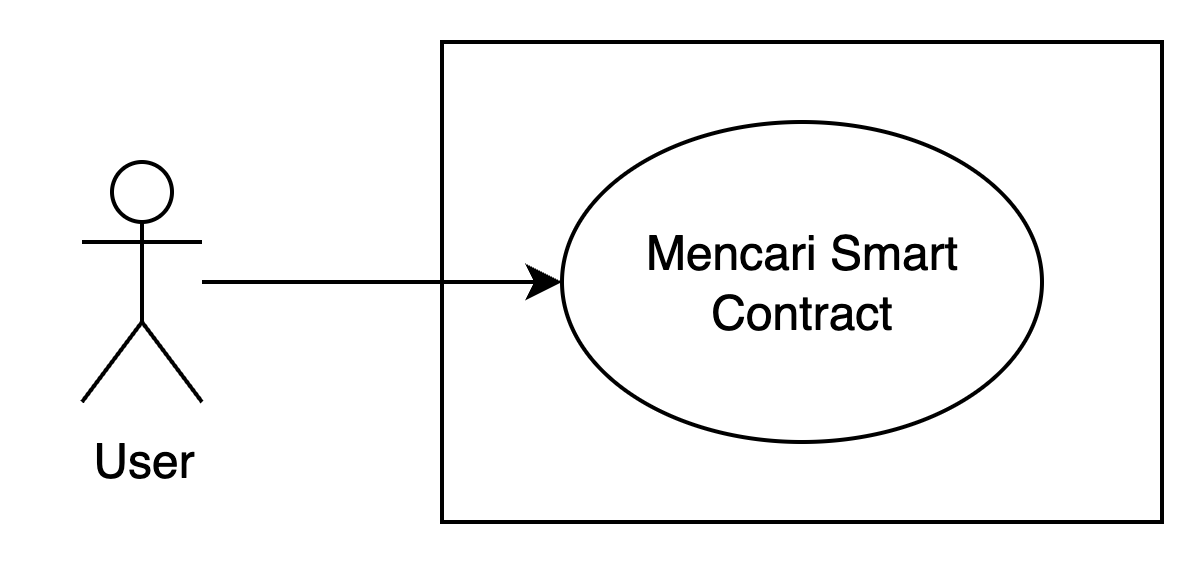
\includegraphics[width=0.7\textwidth]{resources/chapter-3/use-case.png}
	\caption{Use Case Diagram}
	\label{image:usecase}
\end{figure}

\begin{table}[h]
	\caption{Use Case}
	\label{tabel:use-case}
	\vspace{0.25cm}
	\begin{center}
		\begin{tabular}{|c|p{0.25\linewidth}|p{0.55\linewidth}|}
			\hline
			\textbf{ID} & \textbf{Use Case}                  & \textbf{Deskripsi}                                                                                                                                                       \\ \hline
			UC01        & Mencari Smart Contract             & Sistem memberikan data Smart Contract hasil dari pencarian berdasarkan query yang diberikan oleh pengguna. Pengguna dapat memasukkan query pencarian dalam bahasa alami. \\ \hline
			% UC02        & Mendapatkan Address Smart Contract & Sistem memberikan detail address dari Smart Contract yang dipilih oleh pengguna.                                                                                         \\ \hline
		\end{tabular}
	\end{center}
\end{table}

\subsubsection{Kebutuhan Fungsional}

Berdasarkan rumusan Use Case dan karakteristik pengguna, terdapat beberapa kebutuhan fungsional dari sistem yang perlu dipenuhi. Kebutuhan ini akan dibagi menjadi dua perspektif, yaitu perspektif pengguna, yaitu kebutuhan yang berinteraksi dengan pengguna, dan perspektif sistem, yaitu kebutuhan yang perlu dipenuhi untuk sistem beroperasi sesuai fungsional. Seluruh kebutuhan fungsional ini mencakup semua fitur dan fungsi yang perlu ada dalam sistem. Kebutuhan fungsional dari perspektif pengguna akan memiliki sebuah identifikasi yang diawali dengan huruf F-USR lalu diikuti dengan dua angka, sedangkan kebutuhan fungsional dari perspektif sistem akan memiliki sebuah identifikasi yang diawali dengan huruf F-SYS lalu diikuti dengan dua angka juga. Berikut adalah daftar kebutuhan fungsional dari perspektif pengguna yang diidentifikasi:

\begin{table}[ht]
	\caption{Kebutuhan Fungsional Perspektif Pengguna}
	\vspace{0.25cm}
	\begin{center}
		\begin{tabular}{|c|l|}
			\hline
			\textbf{ID} & \textbf{Penjelasan}                                      \\ \hline
			% F-USR01     & Sistem harus menyediakan antarmuka bagi pengguna untuk   \\ & memasukkan query pencarian \\ \hline
			F-USR01     & Sistem harus dapat menerima input query pencarian dari   \\ & pengguna dalam bahasa alami \\ \hline
			F-USR02     & Sistem harus memberikan hasil pencarian Smart Contracts  \\ & yang relevan dengan query pencarian yang diberikan \\ \hline
			F-USR03     & Sistem harus memberikan detail informasi dari Smart      \\ & Contract yang dipilih oleh pengguna \\ \hline
			% F-USR04     & Sistem harus dapat menerima input jumlah Smart Contracts \\ & yang dicari \\ \hline
		\end{tabular}
	\end{center}
\end{table}

\break

Selain kebutuhan fungsional dari perspektif pengguna, sistem juga memiliki kebutuhan fungsional dari perspektif sistem. Kebutuhan ini diperlukan untuk memastikan bahwa sistem dapat beroperasi dengan baik dan memenuhi semua fungsionalitas yang diharapkan, walau tanpa interaksi langsung dengan pengguna. Berikut adalah daftar kebutuhan fungsional dari perspektif sistem yang diidentifikasi:

\begin{table}[ht]
	\caption{Kebutuhan Fungsional Perspektif Sistem}
	\vspace{0.25cm}
	\begin{center}
		\begin{tabular}{|c|l|}
			\hline
			\textbf{ID} & \textbf{Penjelasan}                                         \\ \hline
			F-SYS01     & Sistem mampu mengekstraksi data Smart Contracts dari        \\ & Blockchain Ethereum Mainnet \\ \hline
			F-SYS02     & Sistem dapat mengimpor, menyimpan, dan mengelola data       \\ & Smart Contracts yang telah diekstraksi dan diperkaya  \\ \hline
			F-SYS03     & Sistem harus menyediakan fungsionalitas untuk melihat dan   \\ & mendapatkan data Smart Contracts yang sudah disimpan  \\ \hline
			F-SYS04     & Sistem dapat mengklasifikasikan Smart Contracts berdasarkan \\ & fungsionalitas dan semantik \\ \hline
			% F-SYS05     & Sistem harus menyediakan API yang memungkinkan pengguna     \\ & untuk berinteraksi dengan sistem sesuai fungsionalitas \\ \hline
			% F08 -> memfasilitasi pengguna dalam menggunakan kembali Smart Contracts yang ditemukan dengan menyediakan informasi yang dapat ditindaklanjuti.
		\end{tabular}
	\end{center}
\end{table}

% F01
% "Sistem harus dapat mengekstraksi kode sumber (jika tersedia), bytecode, ABI, alamat kontrak, dan tanggal pembuatan Smart Contracts dari Blockchain Ethereum Mainnet."
% "Sistem harus menyediakan opsi untuk mengekstraksi data Smart Contracts secara terjadwal (misalnya, harian) atau berdasarkan permintaan pengguna."
% (Jika relevan) "Sistem harus memungkinkan pengguna untuk memfilter Smart Contracts yang akan diekstraksi berdasarkan rentang tanggal deployment."

% F02 (+F03)
% "Sistem harus dapat menyimpan data Smart Contracts yang telah diekstraksi (sesuai F01) ke dalam sebuah database."
% "Sistem harus menyediakan fungsionalitas untuk melihat detail, memperbarui metadata (jika diizinkan), dan menghapus (secara logis/fisik) data Smart Contracts yang tersimpan."
% Jika "diperkaya" adalah fungsi sistem: "Sistem harus dapat memperkaya data Smart Contracts dengan [sebutkan jenis data pengayaan, misal: tag kategori, hasil analisis statis awal] setelah proses ekstraksi."

% F03 -> F04
% "Sistem harus dapat secara otomatis mengklasifikasikan Smart Contracts ke dalam kategori fungsionalitas yang telah ditentukan sebelumnya (misalnya, DeFi, NFT, Gaming, DAO) berdasarkan analisis [sebutkan dasar analisis, misal: pola kode, metadata]."
% "Sistem harus memungkinkan pengguna (misalnya, admin) untuk meninjau dan mengoreksi hasil klasifikasi otomatis."
% "Sistem harus memungkinkan pengguna (misalnya, admin) untuk menambahkan atau memodifikasi kategori klasifikasi fungsionalitas dan semantik."

% \subsubsection{Kebutuhan Non-Fungsional}

% Selain kebutuhan fungsional, sistem ini juga harus memenuhi berbagai kebutuhan non-fungsional agar kualitas dan keandalan sistem terjaga. Seluruh kebutuhan non-fungsional akan diberikan ID yang diawali dengan huruf NF lalu diikuti dengan dua angka. Kebutuhan non-fungsional mencakup aspek-aspek berikut:

% \begin{itemize}
% 	\item \textbf{Kinerja (Performance)}: Waktu respons pencarian tidak lebih dari 2 detik untuk kueri dengan bahasa alami.
% 	\item \textbf{Keandalan (Reliability)}: Tingkat ketersediaan (uptime) sistem minimal 99,5\% per bulan.
% 	\item \textbf{Keamanan (Security)}: Semua akses API dan UI harus melalui otentikasi, serta data kontrak harus dienkripsi saat penyimpanan dan transmisi.
% 	\item \textbf{Skalabilitas (Scalability)}: Sistem mampu menangani peningkatan volume data kontrak hingga 10x tanpa degradasi signifikan.
% 	\item \textbf{Keterpakai-an (Usability)}: Antarmuka pengguna intuitif dan dapat digunakan tanpa pelatihan khusus.
% 	\item \textbf{Keterpeliharaan (Maintainability)}: Kode modular dan terdokumentasi, memungkinkan tim pengembang melakukan perbaikan dan penambahan fitur dengan cepat.
% \end{itemize}

% masih ngasal

% \begin{table}[h]
% 	\caption{Kebutuhan Non-Fungsional Sistem}
% 	\vspace{0.25cm}
% 	\begin{center}
% 		\begin{tabular}{|c|p{0.85\linewidth}|}
% 			\hline
% 			\textbf{ID} & \textbf{Penjelasan} \\ \hline
% 			NF01 & Sistem harus memiliki waktu respons pencarian tidak lebih dari 2 detik untuk kueri bahasa alami \\ \hline
% 			NF02 & Sistem harus memiliki tingkat ketersediaan (\textit{uptime}) minimal 99,5\% per bulan \\ \hline
% 			NF03 & Semua akses API dan UI harus melalui otentikasi \\ \hline
% 			NF04 & Data kontrak harus dienkripsi saat penyimpanan dan transmisi \\ \hline
% 			NF05 & Sistem harus mampu menangani peningkatan volume data kontrak hingga 10x tanpa degradasi signifikan \\ \hline
% 			NF06 & Antarmuka pengguna harus intuitif dan dapat digunakan tanpa pelatihan khusus \\ \hline
% 			NF07 & Kode harus modular dan terdokumentasi, memungkinkan tim pengembang melakukan perbaikan dan penambahan fitur dengan cepat \\ \hline
% 			NF08 & Sistem harus memiliki dokumentasi yang jelas dan lengkap untuk pengguna dan pengembang \\ \hline
% 		\end{tabular}
% 	\end{center}
% \end{table}

